\documentclass[midd]{thesis}

\usepackage{graphicx}
\usepackage{times}

\bibliographystyle{plain}

\title {Combating Fraud By Leveraging Machine Learning and Human Behavior}

\author {Casey Astiz}
\adviser {Professor Michael Linderman}

\begin{document}

\maketitle
\pagenumbering{roman}

\begin{abstract}
I am writing about fraud and how to detect it! Wooh!
\end{abstract}

\begin{acknowledgements}
Thank you Professor Linderman and Professor Scharstein!!
\end{acknowledgements}

\contentspage
\tablelistpage   % comment this out if you don't have any tables
\figurelistpage

\normalspacing \setcounter{page}{1} \pagenumbering{arabic}

\chapter{Introduction}
\label{sec:intro}
%This thesis has many chapters.  For more on Alice see
%Chapter~\ref{sec:alice}, and in particular Section~\ref{sec:reproach}.

In today's world, there are more and more ways to pay for goods and services. Cash is a way of the past; mobile, peer to peer, and online payments are the way of the future. While these convenient payment methods are very exciting, the additional methods of payment lead to more gaps in security, in particular fraud. Fraudsters have taken advantage of every system in some form or another, and it is the financial institution's job to block or detect these fraudsters or else deal with the payments. For reference, credit card fraud through online payments in Australia hit \$476 million in 2017, rising \$58 million from the year before \cite{Wang2018}.

The main purpose of this thesis is to investigate current methods of fraud detection and implement one or more of those methods in a financial context. I will discuss the most prevalent methods for fraud detection are currently, as well as past fraud detection methods. Fraud detection is a difficult field of study because it falls in the subset of anomaly detection and has very skewed classes as more transactions are not fraud than are fraud, and the classification of fraud is always changing. In order to build an effective fraud detector, it must be adaptive to new patterns and categories of fraud that are developing as fraudsters find new methods to deceive the system.

The main focus of this thesis will be a review of different methods used in the industry in the past and today for fraud detection, as well as my own implementation using some dataset of transactions to be determined. This background section will include information from published research papers as well as information I learned from interviewing people at different companies in this field to provide some context for the literature review. Comparing business interactions with fraud to published research in the field will allow me to somewhat analyze the performance of different machine learning methods in real life versus a research context.  

Chapter~\ref{sec:background} discusses past and current research into the field of fraud detection. Chapter~\ref{sec:context} gives context for the problem at hand, synthesizing the information I learned from interviewing professionals in the fraud world. In Chapter~\ref{sec:impl}, I describe the methodology and experiments I ran.

This thesis will outline the problem at hand, describe current solutions to the problem, explain an implementation of a solution, provide context with some interviews of experts in the field, and conclude.



\pagebreak

\chapter{Modern Day Fraud}
\label{sec:background}
The text for Section 1 goes here.


\section{Credit Card Fraud}



\subsection{Online Payments Fraud}


% might make this its own chapter
\section{Current Research}


\section{The Human Element}

In this section I will discuss some game theory and behavioral elements of fraud and ways of eliminating frauds and fraudsters.



\noindent
%where $\omega$ is the frequency of the plasmon, $c$ is the speed of
%light, $\varepsilon_m$ is the dielectric constant of the metal,
%$\varepsilon_i$ is the dielectric constant of neighboring insulator,
%and $\varepsilon_{air}$ is the dielectric constant of air.
%Equation~\ref{eqn:sampleEqn} makes this perfectly clear.
%See also Figure~\ref{fig:myfig} for an illustration.
%
%
%\begin{figure}
%\centering
%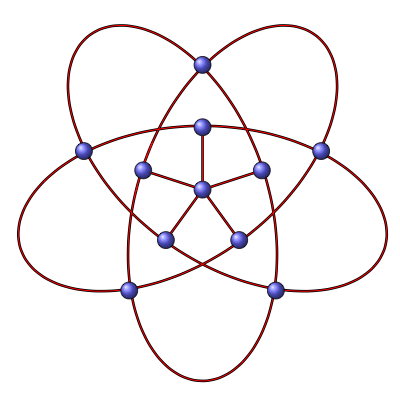
\includegraphics[width=0.75\textwidth]{graph.png}
%\caption{My figure.}
%\label{fig:myfig}
%\end{figure}

\pagebreak
\chapter{ Fraud in Context}
\label{sec:context}

\section{ Interviews from Professionals}

This section will be about what professionals are doing in the fraud field.

\section{ Research Versus Reality}

This section I will compare whatever I find out from professionals to the most modern research on this topic. I assume research will be slightly behind what these professionals are dealing with and how they are solving these problems.

%(As promised in Chapter~\ref{sec:intro}, here it gets interesting.)

\pagebreak
\chapter{Implementing a Fraud Detection System}
\label{sec:impl}


\section{Model}

This section is where I will talk about the overall system I am planning on implementing.

\section{Experiment}

\subsection{Hypothesis}

\subsection{Data}

\subsection{Methods}

LOTS of Machine Learning incorporated into bigger fraud detection and rule based learning systems! Overall system will be discussed in Model section.

\subsection{Results}

This section will be full of tables and figures. There will probably also be an appendix with the entire set of experiments run. The most interesting or a subset of the experimental runs will be in a table in this section.

\subsection{Discussion}

This section will compare my hypothesis to the results, as well as my results to the model I'm basing it off of. I also plan on adding any notes I learn along the way of this implementation.
\pagebreak
\chapter{Further Applications}


\section{Anomoly Detection}

\subsection{Cell Phone Fraud}

\subsection{Biometric Fraud}

\subsection{Bioinformatics}

\pagebreak
\chapter{Conclusions}


%\appendix
%\chapter{Chapter 1 of appendix}
%Appendix chapter 1 text goes here

\bibliography{thesis}

\end{document}
